\chapter{Nền tảng lý thuyết}
\section{Bitcoin}
Các hình thức thương mại trên Internet ngày này hầu như đều dựa vào một tổ chức 
bên thứ ba đáng tin cậy để xử lý các hoạt động thanh toán điện tử. Tuy rằng sau 
nhiều năm phát triển, các tổ chức bên thứ ba này đều đã nâng cao mức độ tin cậy, 
an toàn nhưng đa số vẫn còn tồn tại những điểm yếu: không thể tránh khỏi những 
tranh chấp, phí trung gian, đòi hòi phải cung cấp các thông tin cá nhân... Và 
Bitcoin - hệ thống tiền điện tử ngang hàng (A Peer-to-Peer Electronic Cash System) 
được sinh ra để giải quyết các vấn đề trên \cite{BitcoinPaper}.
\subsection{Sơ lược thông tin về Bitcoin}
Khi so sánh với tiền tệ truyền thống, Bitcoin có hình thức và cách thức hoạt 
động khác biệt. Bitcoin không hề có bất kỳ một tổ chức tập trung nào để quản 
lý, thay vào đó, Bitcoin sử dụng mạng ngang hàng để hoạt động \cite{Bitcoin1}.
\\\\
Trong cách viết, Bitcoin được hiểu như một hệ thống, giao thức hoặc một cộng 
động, cụ thể trong phạm vi luận văn này, Bitcoin được hiểu là một hệ thống. Còn 
BTC được hiểu là một tài sản hoặc một đơn vị tiền tệ.\\\\
BTC được sinh ra bằng cách sử dụng các tài nguyên phần cứng và năng lượng (CPU, 
GPU, phần cứng ASIC, điện năng...) để đi giải một ``câu đố mã hóa'', phần thưởng 
cho người chiến thắng chính là BTC. Trong thời gian đầu (210.000 block đầu tiên) 
(tham khảo về block ở mục 3.1.5), phần thưởng là 50 BTC và các giai đoạn sau sẽ giảm 
dần đi một nửa (25 BTC, 12.5 BTC ...) cứ sau khoảng 210.000 block. Đặc biệt, số 
lượng BTC là hữu hạn và chính xác là 21 triệu BTC, ước tính đến năm 2140 lượng 
BTC khai thác sẽ cạn kiệt \cite{Bitcoin2}. Cũng chính tính chất này là một trong 
những yếu tố tạo nên giá trị của BTC, vì bị giới hạn số lượng nên BTC có tính 
khan hiếm và không bị lạm phát, các tính chất này khác biệt so với tiền tệ 
truyền thống và được ví như vàng 2.0 - vàng của mạng Internet.\\\\
Ngoài các yếu tố vượt trội trên, Bitcoin còn được xây dựng là một hệ thống có 
tính chất ẩn danh, các địa chỉ chứa BTC đều là những dãy ký tự trừu tượng, không 
có ý nghĩa về mặt xác minh cá nhân và rất khó để biết ai là chủ nhân thật sự của 
một địa chỉ. Mặc dù, Bitcoin có tính ẩn danh nhưng tất cả những giao dịch trên 
hệ thống đều được công khai, điều đó có nghĩa là một giao dịch phải được sự xác 
minh về tính hợp lệ của đa số các thành viên trong mạng. Việc xác minh dựa vào các 
quan hệ, cấu trúc liên quan đến toán học, mật mã... \cite{Bitcoin1, BitcoinPaper}\\\\
Tính công khai của Bitcoin được thể hiện ở quá trình xác minh các giao dịch, 
ngoài ra nó còn được thể hiện ở phương diện kỹ thuật, các mã nguồn lập trình 
và các đoạn lập trình đều được công khai.\\\\
Đơn vị giao dịch, BTC có thể được chia thành nhiều đơn vị nhỏ hơn, tối thiểu 
là đơn vị $Satoshi$. Cụ thể $1 \, Satoshi = 100 \, \mu BTC = 0.00000001 \, BTC$ 
hoặc $1 \, BTC = 100.000.000 \, BTC$ \cite{Bitcoin3}.
\subsection{Máy chủ nhãn thời gian - Timestamp Server}
Máy chủ nhãn thời gian hoạt động bằng cách lấy giá trị băm (hash) của block 
liền trước và thông tin của block hiện tại, cho qua hàm băm để được một giá trị 
băm mới. Giá trị băm sau khi được tính toán sẽ được công bố rộng rãi và giá trị 
băm này chứng minh rằng block tồn tại, các block được nối với nhau thành một 
chuỗi xác định.\\
\begin{figure}[h!]
\centering
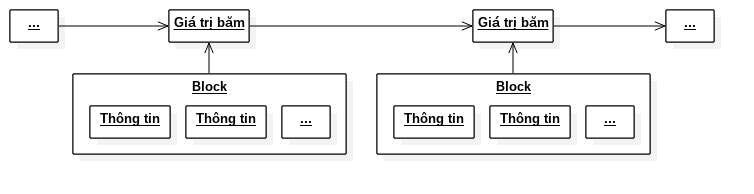
\includegraphics[height=1.45in, keepaspectratio=true]{timestampserver.png}
\caption{Máy chủ nhãn thời gian}
\end{figure}
\subsection{Giao dịch - Transaction (trên Blockchain)}
Bitcoin tổ chức các giao dịch bằng cách xây dựng một chuỗi các chữ ký số. Một 
địa chỉ có chứa một lượng BTC được gọi là một chủ sở hữu, một chủ sở hữu 
chuyển một lượng BTC cho một chủ sở hữu khác - người thụ hưởng - bằng cách ký 
lên giá trị băm, trong đó giá trị băm là kết quả sau khi đi qua hàm băm
của tổ hợp giá trị băm giao dịch trước với địa chỉ người thụ hưởng.\\
\begin{figure}[h!]
\centering
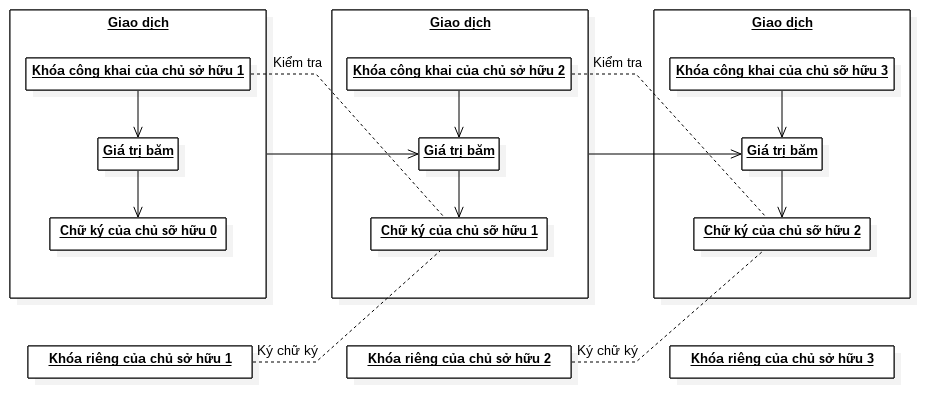
\includegraphics[height=2.45in, keepaspectratio=true]{transaction.png}
\caption{Giao dịch}
\end{figure}
\subsection{Proof-of-Work}
Proof-of-Work được hiểu là bằng chứng để chứng minh quá trình lao động, nó dùng 
để kiểm tra quá trình tạo ra kết quả hợp lệ là một quá trình ``lao động'' có 
sử dụng và tiêu tốn tài nguyên.\\\\
Proof-of-Work được sử dụng trong Bitcoin có cơ chế dựa trên hàm băm, ví dụ như 
SHA-256. Quá trình proof-of-work là quá trình đi tăng một con số - gọi là số 
$nonce$ - sao cho giá trị băm của số $nonce$ này cho kết quả đầu ra phải thỏa 
mãn tồn tại $n$ bit 0 ở vị trí đầu, với $n$ xác định và được gọi là số bit 0 
yêu cầu.
\subsection{Blockchain}
Blockchain được hình thành dựa trên sự kết hợp giữa máy chủ nhãn thời gian và 
proof-of-work. Blockchain là một chuỗi các block được kết nối một cách luận lý 
với nhau thông qua các mỗi quan hệ toán học và mật mã, các quan hệ này đảm bảo 
cho hệ thống luôn đúng đắn, không thể sửa và dễ dàng để kiểm tra. Block mới được 
sinh ra phải dựa trên quá trình proof-of-work.\\\\
Quá trình hình thành blockchain được bắt đầu bằng proof-of-work, các peer sẽ đi
tìm số $nonce$ sao cho sau khi cho qua hàm băm kết quả đạt được là một giá trị 
băm thỏa mãn số bit 0 yêu cầu. Số $nonce$ vừa được tìm ra sẽ được đưa và block
mới cùng với các thông tin khác như: thông tin các giao dịch, giá trị băm của 
block kề trước... Tiếp tục như vậy, các block mới được sinh ra và được kết nối 
với block cuối cùng của chuỗi.\\
\begin{figure}[h!]
\centering
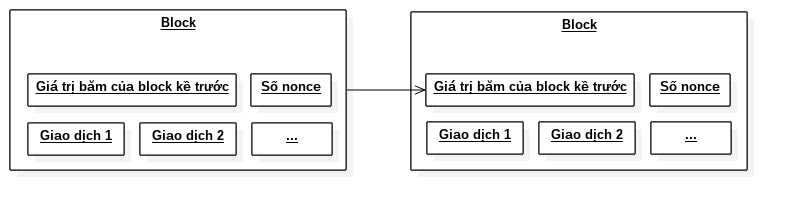
\includegraphics[height=1.5in, keepaspectratio=true]{blockchain.png}
\caption{Blockchain}
\end{figure}\\
Vì hệ thống có tính phân tán nên trên toàn mạng sẽ có nhiều phiên bản của blockchain,
cũng chính vì thế để giải quyết tính đồng nhất, chỉ blockchain có độ dài lớn 
nhất mới được xem là blockchain hợp lệ. Đồng thời để kiểm soát được tốc độ sinh
block mới, hệ thống sẽ quy định một độ khó, nếu toàn mạng có tốc độ sinh block 
(số block được sinh ra trong một giờ đồng hồ) cao hơn mức quy định, độ khó sẽ tăng lên 
để điều chỉnh lại tốc độ của toàn mạng.
\subsection{Mạng - Network}
Mỗi thành viên (máy tính, phần cứng ASIC, thiết bị di dộng... ) khi tham gia vào quá 
trình tính toán của toàn mạng thì sẽ được xem như một node. Toàn mạng sẽ hiện thực hệ 
thống bằng cách thực hiện các bước như sau:
\begin{enumerate}
\item Một giao dịch mới được truyền đi cho tất cả các node (broadcast).
\item Mỗi node sẽ lựa chọn và thu thập các giao dịch để đưa vào block.
\item Mỗi node sẽ thực hiện proof-of-work, tìm ra số $nonce$.
\item Khi một node hoàn thành proof-of-work, node này sẽ đóng block và truyền 
đi toàn tất cả các node khác.
\item Các node khác sẽ kiểm tra thông tin của block nhận được (thông tin các 
giao dịch, thông tin proof-of-work...) và chấp nhận block này nếu tất cả 
các thông tin đều được kiểm tra chính xác.
\item Các node sẽ thể hiện sự chấp nhận của mình bằng cách thực hiện proof-of-work 
để sinh ra block mới block này sẽ được gắn vào liền sau block mà node đã chấp nhận 
(thêm giá trị băm của block trước mà node chấp nhận vào trong block mới sinh ra).
\end{enumerate}
Lưu ý, một giao dịch mới không nhất thiết phải được truyền đến tất cả các node. 
Chỉ cần việc truyền đến số node đủ nhiều để đảm bảo việc sẽ được đưa vào một block 
và được đóng trong blockchain với độ dài lớn nhất. Cũng như vậy đối với block, 
block không nhất thiết phải được truyền đến tất cả các node, khi một node nhận 
được một block kế block bị thiếu, bằng quá trình kiểm tra node có thể biết được 
và yêu cầu các node khác trong mạng gửi cho node này block bị thiếu sót.
\subsection{Phần thưởng khích lệ}
Trong tập các giao dịch được đóng trong một block sẽ luôn tồn tại một giao dịch 
đặc biệt, giao dịch này khác với các giao dịch bình thường, nó không có người chủ 
sở hữu mà chỉ có người thụ hưởng. Điều này giải thích cách mà BTC mới được sinh 
ra, cứ mỗi block được tìm ra nhờ quá trình proof-of-work sẽ có một lượng BTC 
được sinh ra và chính là phần thưởng cho người tạo ra block - người tạo ra block 
này cần được toàn mạng xác minh proof-of-work và công nhận là hợp lệ, địa chỉ 
người thụ hưởng chính là địa chỉ của người tạo ra block.\\\\
Ngoài ra, phần thưởng khích lệ khi tạo ra được một block còn bao gồm cả phí giao 
dịch từ các giao dịch đã được đóng trong block. Phí giao dịch thường rất nhỏ và
không đáng kể ở thời điểm hiện tại.
\subsection{Tổ chức lưu trữ thông tin giao dịch}
Đối với các node là các hệ thống máy tính lớn, khả năng lưu trữ và xử lý mạnh thì 
việc lưu một block với đầy đủ các thông tin không gặp nhiều vấn đề. Nhưng đối 
với các thiết bị di động hoặc các thiết bị khác với tài nguyên lưu trữ và xử lý 
tương đối hạn hẹp thì việc lưu một blockchain đầy đủ là khá khó khăn.\\\\
Cây Merkle là một cấu trúc tổ chức dữ liệu, trong đó giá trị của node cha sẽ 
là kết quả hàm băm tất cả các giá trị (nhãn hoặc dữ liệu) của nốt con. Các nốt 
không phải lá thì giá trị sẽ là nhãn - kết quả hàm băm, các nốt lá sẽ có giá trị 
là dữ liệu cần được tổ chức.\\\\
Bitcoin sử dụng cây Merkle để tổ chức các giao dịch, nốt cao nhất của cây được 
gọi là giá trị băm gốc (Root hash) và giá trị này sẽ được lưu vào block. Ở đây,
ta thấy việc thay đổi bất kỳ một giá trị nào trong cây cũng sẽ dẫn đến việc thay 
đổi giá trị băm gốc, vì thế giá trị băm gốc khi được lưu vào block nó có chức 
năng dùng để kiểm tra lại các giao dịch trong block đó là toàn vẹn hay không.\\
\begin{figure}[h!]
\centering
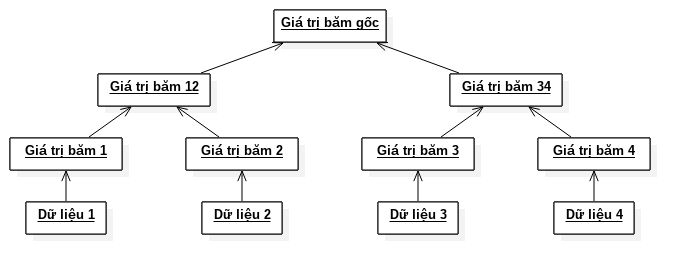
\includegraphics[height=2.25in, keepaspectratio=true]{merkletree.png}
\caption{Cây Merkle}
\end{figure}
\begin{figure}[h!]
\centering
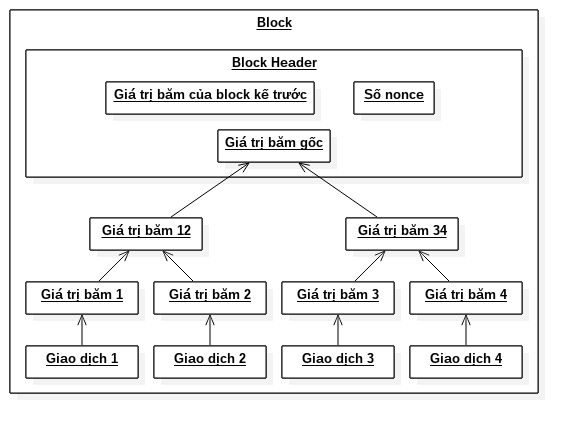
\includegraphics[height=3.75in, keepaspectratio=true]{block.png}
\caption{Cấu trúc tổ chức giao dịch trong một block}
\end{figure}\\
Một node với tài nguyên hạn chế khi muốn lưu blockchain không nhất thiết phải 
lưu đầy đủ thông tin của từng block trong blockchain, thay vào đó node có thể 
lược bỏ các thông tin về giao dịch được đóng trong block và chỉ lưu giá trị băm 
gốc của các giao dịch này. Điều này làm giảm chi phí về lưu trữ nhưng vẫn đảm 
bảo được tính toàn vẹn, khi muốn xác minh bất kỳ giao dịch nào, node chỉ cần 
yêu cầu các giao dịch trong block và tính toán lại giá trị băm gốc, nếu giá trị 
băm nào giống với giá trị băm gốc được lưu nghĩa là các giao dịch hoàn toàn hợp 
lệ.
\section{Một số khái niệm về tài chính}
\subsection{Phiên giao dịch và các giá trị cơ bản}
Gọi $T$ là một mốc thời gian bất kỳ, $P$ là khoảng thời gian được chọn là một 
phiên giao dịch. Ta có thể nói một cách đơn giản là phiên giao dịch được mở tại 
thời điểm $T$ và được kết thúc tại thời điểm $T + P$.\\\\
Cụ thể, giả sử chọn mốc mở phiên là 9:00am và phiên giao dịch có thời hạn là 
30 phút, điều đó có nghĩa là kết thúc phiên giao dịch sẽ là 9:30am.\\\\
Các thông tin của một phiên giao dịch:
\begin{itemize}
\item Giá mở phiên: là giá bán của một giao dịch gần nhất sau thời điểm $T$. Ví 
dụ tại thời điểm 9:01am có một giao dịch bán 1 BTC là \$779 và trong khoảng thời 
gian 9:00am đến 9:01am không hề có bất kỳ giao dịch nào khác ngoại trừ giao dịch 
này, thì ta có thể nói giá mở phiên sẽ là \$779.
\item Giá đóng phiên: là giá bán của một giao dịch gần nhất trước thời điểm 
$T + P$.
\item Giá phiên cao nhất: là giá bán cao nhất của một giao dịch trong khoảng 
thời gian diễn ra phiên giao dịch, cụ thể là từ thời điểm $T$ đến thời điểm 
$T + P$. Ví dụ, trong khoảng thời gian 9:00am (thời điểm mở phiên) đến thời gian 
9:30am (thời điểm đóng phiên) có một giao dịch BTC với giá là \$801 và là giao 
dịch có giá trị cao nhất. Vậy ta có thể nó giá phiên cao nhất là \$801.
\item Giá phiên thấp nhất: là giá bán thấp nhất của một giao dịch trong khoảng 
thời gian diễn ra phiên giao dịch, cụ thể là từ thời điểm $T$ đến thời điểm $T + P$.
\item Lượng giao dịch: tổng giá trị USD được dùng để  mua/bán BTC trong một phiên 
giao dịch.
\item Trung bình giao dịch: giá trị USD trung bình của tất cả các giao dịch diễn 
ra trong khoảng thời gian một phiên giao dịch.
\end{itemize}
\subsection{Overbought và Oversold}
Overbought dùng để định nghĩa trường hợp thị trường có mức cầu cao hơn mức cung, 
điều này làm đẩy giá của tài sản giao dịch lên cao vượt qua mức chính đáng. Ví 
dụ, trên tất cả các giao dịch có hơn 80\% lệnh là đặt mua và dưới 20\% là lệnh 
đặt bán, trường hợp này được xem là overbought.\\\\
Ngược lại, oversold dùng để định nghĩa trường hợp thị trường có mức cung cao hơn 
mức cầu, điều này làm kéo giá của tài sản giao dịch xuống thấp vượt mức chính 
đáng.
\subsection{Chỉ số dao động ngẫu nhiên - Stochastic Oscillator}
Đại lượng dùng để đo xu hướng mua/bán của thị trường tại thời điểm phiên $x$ 
thông qua $n$ phiên trước đó. Giả sử:\\\\
\tab $L_{n} = $ giá phiên thấp nhất trong $n$ phiên\\
\tab $H_{n} = $ giá phiên cao nhất trong $n$ phiên\\
\tab $P(x) = $ giá của ngày $x$\\
\[\%K=\frac{P(x)-L_{n}}{H_{n}-L_{n}}\]
Nếu $ \%K $ nhỏ hơn 20 thì thị trường đang có xu hướng oversold vào và nếu lớn 
hơn 80 thì thị trường đang có xu hướng overbought.
\subsection{Tỉ lệ thay đổi - Rate of Change}
Đại lượng đo sự khác nhau của giá tại phiên thứ $x$ so với $n$ phiên trước đó. 
Giá sử $P(x)$ là giá của phiên thứ $x$ thì:
\[ ROC_{n}(x)=\frac{P(x)-P(x-n)}{P(x-n)}\]
Nếu $ROC > 0$ thì giá thị trường đang có xu hướng đi lên (tăng giá).
Ngược lại, với $ROC < 0$ thì giá thị trường đang có xu hướng giảm xuống.
\section{Máy học}
\subsection{Khái niệm cơ bản}
\subsubsection{Máy học}
Máy học có hai cách định nghĩa chính và đang được chấp nhận phổ biến:
\begin{itemize}
  \item Theo Arthur Samuel: \textit{``Là một lĩnh vực nghiên cứu mà nó cung cấp cho
  máy tính khả năng học hỏi mà không cần lập trình một cách tường minh.''}
  \item Theo Tom Mitchell: \textit{``Một chương trình máy tính được chấp nhận
  là học hỏi được kinh nghiệm E bằng cách thực hiện một vài tác vụ T theo phép đo hiệu
  năng P, nếu và chỉ nếu việc thực thi các tác vụ trong T được đo bởi phép đo P
  đem lại kết quả là kinh nghiệm E được cải thiện.''}
\end{itemize}
\subsubsection{Học có giám sát - Supervised Learning}
Chúng ta được cho một tập dữ liệu đã biết với các đầu vào và đầu ra tương ứng
nhau. Ý tưởng là chúng ta sẽ đi tìm mối quan hệ giữa đầu vào và đầu ra, đó 
chính là học có giám sát.\\\\
Vấn đề của học có giám sát được phân loại thành hai
vấn đề chính là hồi quy - regression và phân lớp - classification. Trong vấn đề 
hồi quy, chúng ta sẽ cố gắng dự đoán kết quả đầu ra tiếp theo một cách liên tục, 
nghĩa là chúng ta đi tìm ra một hàm đầu ra liên tục tổng quát với biến là các 
đặc trưng đầu vào. Còn với vấn đề phân lớp, chúng ta thay vì cố gắng dự đoán kết
quả liên tục thì ta sẽ đi dự đoán chúng theo hướng rời rạc, hiểu theo một cách
khác là chúng ta đi tìm một phép phân loại rời rạc cho các biến đầu ra với các 
biến đầu vào.
\subsubsection{Học không giám sát - Unsupervised Learning}
Học không giám sát cho phép chúng ta tiếp cận các vấn đề mà ta chưa hề hoặc biết
rất ít kết quả của chúng ta sẽ trông như thế nào. Chúng ta có thể xây dựng cấu
trúc của dữ liệu mà không cần thiết phải biết mối quan hệ của các biến đó.\\\\
Chúng ta thực hiện việc này dựa trên ý tưởng gom cụm dữ liệu bằng cách xem xét
mối quan hệ giữa các đặc trưng của dữ liệu. Các hướng tiếp cận dựa trên nhưng 
phương pháp như vậy thường được gọi là gom cụm - clustering.
\subsection{Thông số đánh giá}
Có ba tham số cơ bản dùng để xem xét và đánh giá giải thuật trong Máy học.
Ký hiệu:
\begin{itemize}
\item True positive là $TP$
\item False positive là $FP$
\item True negative là $TN$
\item False negative là $FN$
\end{itemize}
Ta có:\\
\[
  Accuracy = \frac{TP+TN}{TP+FP+TN+FN}
\]
\[
  Precision = \frac{TP}{TP+FP}
\]
\[
  Recall = \frac{TP}{TP+FN}
\]
\begin{figure}[h!]
\centering
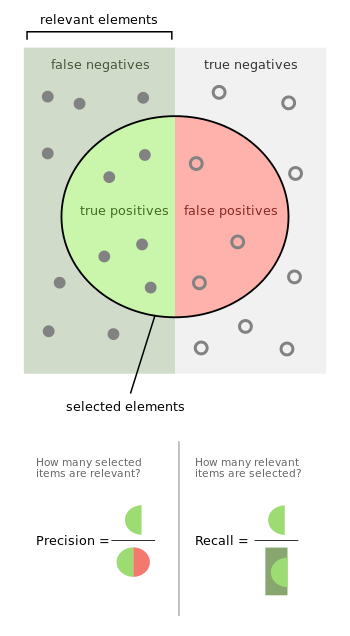
\includegraphics[height=4in, keepaspectratio=true]{precision_recall.png}
\caption{Thông số đánh giá}
\end{figure}
\subsection{Mạng neural - Neural Network}
Học sâu - Deep Learning - là một nhánh của Máy học, đại diện cho hướng tiếp 
cận gần với cái nhìn thực tế, học nhiều cấp và học từ bản chất dữ liệu. Học 
sâu thường giải quyết rất tốt với các loại dữ liệu mang tính ``con người'' 
như hình ảnh, âm thanh ... Để có được những tính chất này, Học sâu đã đưa ra 
các giải thuật mạng neural với cấu tạo nhiều lớp, mỗi lớp lại được cấu tạo từ 
nhiều phần tử nhỏ hơn. Mỗi phần tử bên trong đi giải quyết các phép toán rất 
đơn giản, nhưng khi được ghép nối lại thành một mạng neural hoàn chỉnh chúng có 
thể giải quyết các bài toán phức tạp hơn rất nhiều, điều này hoàn toàn tương tự 
với các hoạt động của bộ não người. \cite{NeuralNetworksandDeepLearning} 
\subsubsection{Cấu trúc một Perceptron}
Một perceptron sẽ có các giá trị đầu vào $x_1, x_2, ...$, giá trị đầu ra sẽ 
là kết quả toán học của các giá trị đầu vào và là một giá trị nhị phân.\\
\begin{figure}[h!]
\centering
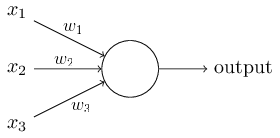
\includegraphics[height=1.5in, keepaspectratio=true]{perceptron_n.png}
\caption{Perceptron}
\end{figure}\\
Một ví dụ, dựa vào hình trên, ta thấy perceptron này có 3 input là 
$x_1, x_2, x_3$ , giả sử đi kèm với mỗi input sẽ có một giá trị trọng 
số $w_1, w_2, w_3$. Output được định nghĩa là 0 và 1, nhận giá trị 0 
khi $\sum_j w_j x_j$ nhỏ hơn giá trị ngưỡng và 1 khi lớn hơn giá trị ngưỡng.\\\\
Biểu diễn đại số:\\
\[
  output = 
  \bigg\{
    _{0 \quad if \, \sum_j w_j x_j \, \leq \, threshold}
    ^{1 \quad if \, \sum_j w_j x_j \, > \, threshold}
\]
Các hàm số như trên được gọi là hàm hoạt động - activation function, có nhiều 
loại hàm hoạt động khác nhau như: $sigmoid , tang ...$ 

\subsubsection{Multilayer Neural Network}
Với một perceptron đơn lẻ, tự thân nó không thể giải quyết được một bài toán 
phức tạp như yêu cầu của mạng neural, vì thế, để giải quyết bài toán phức tạp 
hơn, các perceptron được kết nối với nhau tạo thành một mạng neural.\\\\
MNN được cấu thành bằng cách sắp xếp các perceptron thành 
từng lớp. Các perceptron ở mỗi lớp sẽ kết nối với tất cả các perceptron ở các 
lớp liền kề, lớp những perceptron đầu tiên được gọi là lớp đầu vào (input layer), 
chúng có chức năng tiếp nhận các giá trị đầu vào để cung cấp cho các lớp tiếp 
theo. Các giá trị đầu ra ở lớp trước sẽ chính là các giá trị đầu vào cho 
các perceptron ở lớp tiếp theo. Các perceptron ở lớp cuối cùng được gọi là lớp 
đầu ra (output layer), trong trường hợp này đặc biệt chỉ có duy nhất một 
perceptron ở lớp đầu ra. Còn lại các lớp perceptron khác được gọi là lớp ẩn 
(hidden layer).\\
\begin{figure}[h!]
\centering
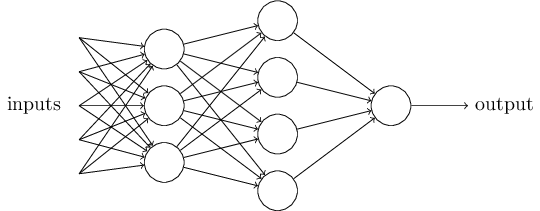
\includegraphics[height=2in, keepaspectratio=true]{multilayerneuralnetwork.png}
\caption{MNN}
\end{figure}\\
Giả sử đầu vào của perceptron là $x_1, x_2, ...$ tương ứng là đó là các trọng 
số $w_1, w_2, ...$. Thêm vào định nghĩa về $bias$, ở đây $bias$ là một giá trị 
đại diện độ lệch của từng perceptron và được ký hiệu $b_1, b_2, ...$. Ta có 
biểu diễn của hàm hoạt động với $bias$:\\
\[
  output = 
  \bigg\{
    _{0 \quad if \, \sum_j w_j x_j + b_i\, \leq \, 0}
    ^{1 \quad if \, \sum_j w_j x_j + b_i\, > \, 0}
\]
Ví dụ:\\
\begin{figure}[h!]
\centering
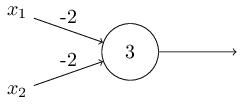
\includegraphics[height=1in, keepaspectratio=true]{exmln.png}
\caption{Ví dụ perceptron với giá trị bias}
\end{figure}\\
Ta có $w_1=w_2=-2$ và $b=3$, khi đó nếu input $x_1=1,\, x_2=0$ suy ra $ 
w_1*x_1+w_2*x_2+b=(-2)*1+(-2)*0+3=1$, ta có thể chọn $threshold=0$ vì $1>0$
nên $output=1$.

\subsubsection{Hàm sigmoid - Sigmoid Function}
Với hàm hoạt động được định nghĩa như trên, giá trị của hàm hoạt động trên lý 
thuyết là không có giới hạn, nghĩa là $output\in\mathbb{R}$. Trong một trường 
hợp cụ thể, với việc sử dụng hàm hoạt động như trên có thể dẫn đến trường hợp 
đầu ra của một perceptron sẽ nhận giá trị rất lớn - giả sử là 1000, những một 
perceptron khác sẽ nhận giá trị rất bé - giả sử 0.001. Vì thế khi đến lớp tiếp 
theo thì gần như perceptron cho kết quả đầu ra là giá trị bé sẽ mất đi độ ảnh 
hưởng và làm mất cân đối cho toàn mạng.\\\\
Do đó để giới hạn giá trị đầu ra của hàm hoạt động chúng ta sẽ sử dụng hàm 
sigmoid. Hàm sigmoid được định nghĩa như sau:\\
\[
  \sigma(z)=\frac{1}{1+e^{-z}}
\]
Với biễu diễn đồ thị:
\begin{figure}[h!]
\centering
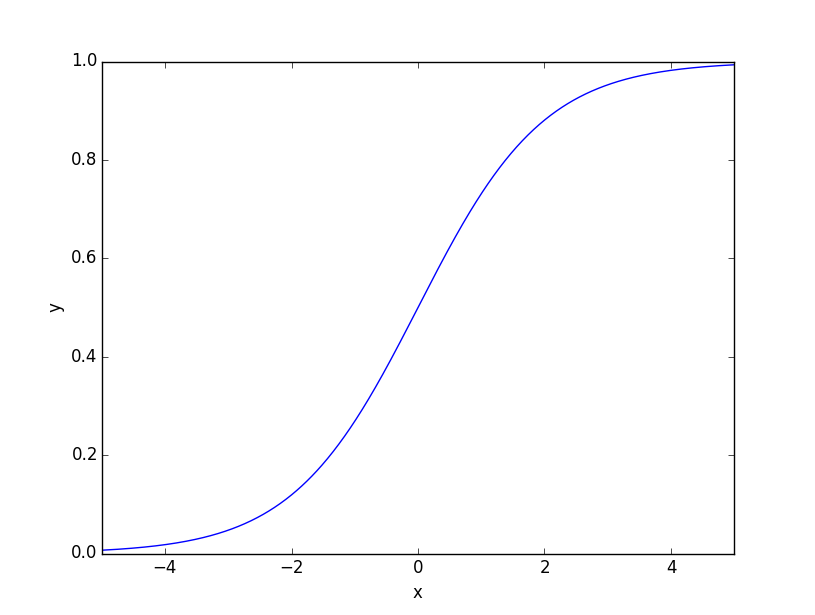
\includegraphics[height=3.85in, keepaspectratio=true]{sigmoid.png}
\caption{Đồ thị hàm sigmoid}
\end{figure}\\
Áp dụng hàm sigmoid vào hàm hoạt động ta có một hàm hoạt động dạng sigmoid và 
khi đó hàm hoạt động của chúng ta của chúng ta sẽ có dạng:\\
\[
  \frac{1}{1+exp(-\sum_j w_j x_j -b)}
\]
Lúc này ta có một hàm hoạt động có giá trị được giới hạn trong khoảng từ 0 đến 
1. Nhưng chú ý, giá trị đầu ra của hàm hoạt động vẫn là giá trị liên tục, để 
rời rạc hóa giá trị đầu ra của hàm hoạt động ta có thể sử dụng một phương pháp 
quen thuộc - sử dụng ngưỡng. Điển hình ta chọn ngưỡng $threshold = 0.5$, nếu 
lớn hơn ngưỡng thì giá trị đầu ra của hàm hoạt động sẽ nhận 1 và ngược lại sẽ 
nhận 0.
\begin{figure}[h!]
\centering
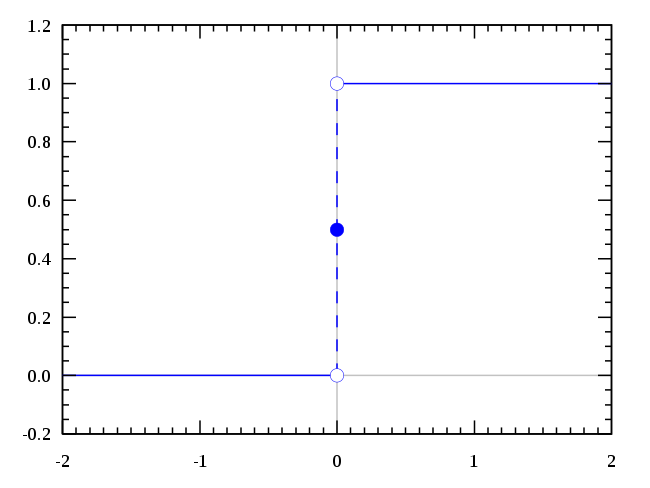
\includegraphics[height=3.5in, keepaspectratio=true]{step.png}
\caption{Đồ thị rời rác hóa hàm sigmoid}
\end{figure}
\subsubsection{Giải thuật lan truyền ngược}
Sau khi đã có xây dựng thành công một mô hình MNN, công việc tiếp theo sẽ là 
cung cấp khả năng tự học hỏi từ đó để bản thân mạng có thể tự xây dựng mô hình 
quyết định và đưa ra các giá trị đầu ra tương ứng với từng trường hợp đầu vào 
cụ thể.\\\\
Cụ thể, khi nhìn lại một MNN với hàm hoạt động là một hàm hoạt động có dạng
sigmoid và các tham số $w, b$, các tham số này chưa có giá trị.  Việc cung 
cấp khả năng tự học hỏi cho mạng chính là cung cấp một giải thuật giúp mạng 
tìm được các tham số $w, b$ với một tập kinh nghiệm - hay tập huấn luyện - 
${x, y}$ cụ thể, trong đó $x$ là giá trị đầu vào và $y$ là giá trị đầu ra 
tương ứng với từng bộ $x$. Giải thuật lan truyền ngược là một giải thuật giúp 
giải quyết vấn đề trên.\\\\
Biểu diễn trọng số, $bias$ và hàm hoạt động:\\\\
Trọng số $w_{jk}^\ell$ là trọng số từ lớp perceptron thứ $k$ của lớp $(\ell-1)$ 
đến perceptron thứ j thuộc lớp thứ $\ell$.
Như hình trên, trọng số xuất phát từ perceptron thứ 4 thuộc lớp thứ 2 và kết 
thúc tại perceptron thứ 2 thuộc lớp thứ 3 được ký hiệu là $w_{24}^3$.\\
\begin{figure}[h!]
\centering
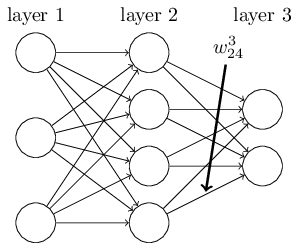
\includegraphics[height=2in, keepaspectratio=true]{exw.png}
\caption{Ký hiệu trọng số}
\end{figure}\\
Tương tự như vậy với $bias$ và hàm hoạt động của perceptron thứ $j$ thuộc lớp 
thứ $\ell$ của mạng sẽ được kí hiệu thứ tự là $b_j^\ell,\,a_j^\ell$. Ví dụ, $bias$ 
của perceptron thứ 3 thuộc lớp thứ 2 sẽ là $b_3^2$ và hàm hoạt động của 
perceptron thứ 1 thuộc lớp thứ 3 sẽ là $a_1^3$.\\
\begin{figure}[h!]
\centering
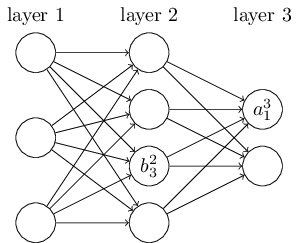
\includegraphics[height=2in, keepaspectratio=true]{exb.png}
\caption{Ký hiệu $bias$}
\end{figure}\\
Biễu diễn ma trận trọng số và vector $bias$:
\begin{itemize}
\item $w$ là ma trận của các giá trị trọng số\\ 
\[ w =
\begin{bmatrix}
w_{11} & \ldots & w_{1k} \\
\vdots & \ddots & \vdots\\
w_{j1} & \ldots & w_{jk}
\end{bmatrix}
\]
\item $b$ là vector của các giá trị $bias$\\ 
\[ b =
\begin{bmatrix}
b_1\\
\vdots\\
b_k
\end{bmatrix}
\]
\item $\sigma$ là hàm sigmoid
\item $a_j=\sigma$ là hàm hoạt động có dạng sigmoid, $a$ là vector của các hàm 
hoạt động\\
\[ a =
\begin{bmatrix}
a_1\\
\vdots\\
a_k
\end{bmatrix}
\]
\end{itemize}
Lúc này ta có biểu diễn toán học đầy đủ của hàm hoạt động:\\
\[
  a_j^\ell=\sigma(\sum_k w_{jk}^\ell a_k^{\ell-1} + b_j^\ell)
\]
Tổng quát phát biểu với dạng:\\
\[
  a^\ell=\sigma(w^\ell a^{\ell-1} + b^\ell)
\]
Để có thể tìm được giá trị của các biến $w$ và $b$, giải thuật lan truyền ngược 
thực hiện bằng cách xuất phát $w$ và $b$ từ các giá trị ngẫu nhiên, thực hiện 
các phép lặp để đưa $w$ và $b$ về giá trị đúng, mỗi lần lặp sẽ có một hàm chi 
phí (cost function) đo đạc độ lệch của giá trị tính toán và giá trị thực tế 
để giúp giải thuật tìm được giá trị hội tụ.\\\\
Biễu diễn hàm chi phí:\\
\[
  C=\frac{1}{2n}\sum_x\|y(x)-a^L(x)\|^2
\]
Ta có thể thấy, dạng hàm số trên tương đồng với định nghĩa độ lệch chuẩn trong 
xác suất thống kê nhưng có một số biến đổi khác biệt. Thay vì giá trị kỳ vọng 
và các giá trị xác suất, hàm chi phí sử dụng giá trị thực tế $y$ của tập dữ 
liệu và giá trị $y=a$ là giá trị $y$ tính toán được từ $x$ với $w$ và $b$. Vậy 
ta có thể hiểu được, hàm chi phí tính toán độ sai lệch của giá trị $a$ so với 
$y$ kỳ vọng thực tế. Do đó, hàm chi phí càng nhỏ thì biểu diễn giá trị của 
MNN sẽ càng gần với thực tế.\\\\
Để tìm được giá trị cực tiểu cho hàm chi phí ta sẽ thực hiện vòng lặp:\\
\[
  w_{ij}^{(\ell)}:=w_{ij}^{(\ell)}-\eta\frac{\delta}{\delta w_{ij}^{(\ell)}}C(w,b)
\]
\[
  b_i^{(\ell)}:=b_i^{(\ell)}-\eta\frac{\delta}{\delta b_i^{(\ell)}}C(w,b)
\]

Trong đó $\eta$ là tỉ lệ học (learning rate), việc hội tụ về giá trị cực tiểu 
với tốc độ và độ chính xác phụ thuộc vào tỉ lệ này.\\\\
Vậy, đi qua một quá trình tìm hiểu về MNN, ta có thể hiểu được việc học hỏi 
kinh nghiệm của mạng cốt lõi vẫn là việc tìm ra bộ $w$ và $b$ tương ứng với 
${x, y}$ của bộ dữ liệu luyện tập, và để tìm ra được $w$ và $b$ ta có thể sử 
dụng giải thuật lan truyền ngược.